\documentclass{article}
\usepackage{amsmath, amssymb, amsthm}
\usepackage{tikz}
\usetikzlibrary{positioning}

\newtheorem{theorem}{Theorem}

\begin{document}

\section*{Overview of Main Results}

\begin{center}
    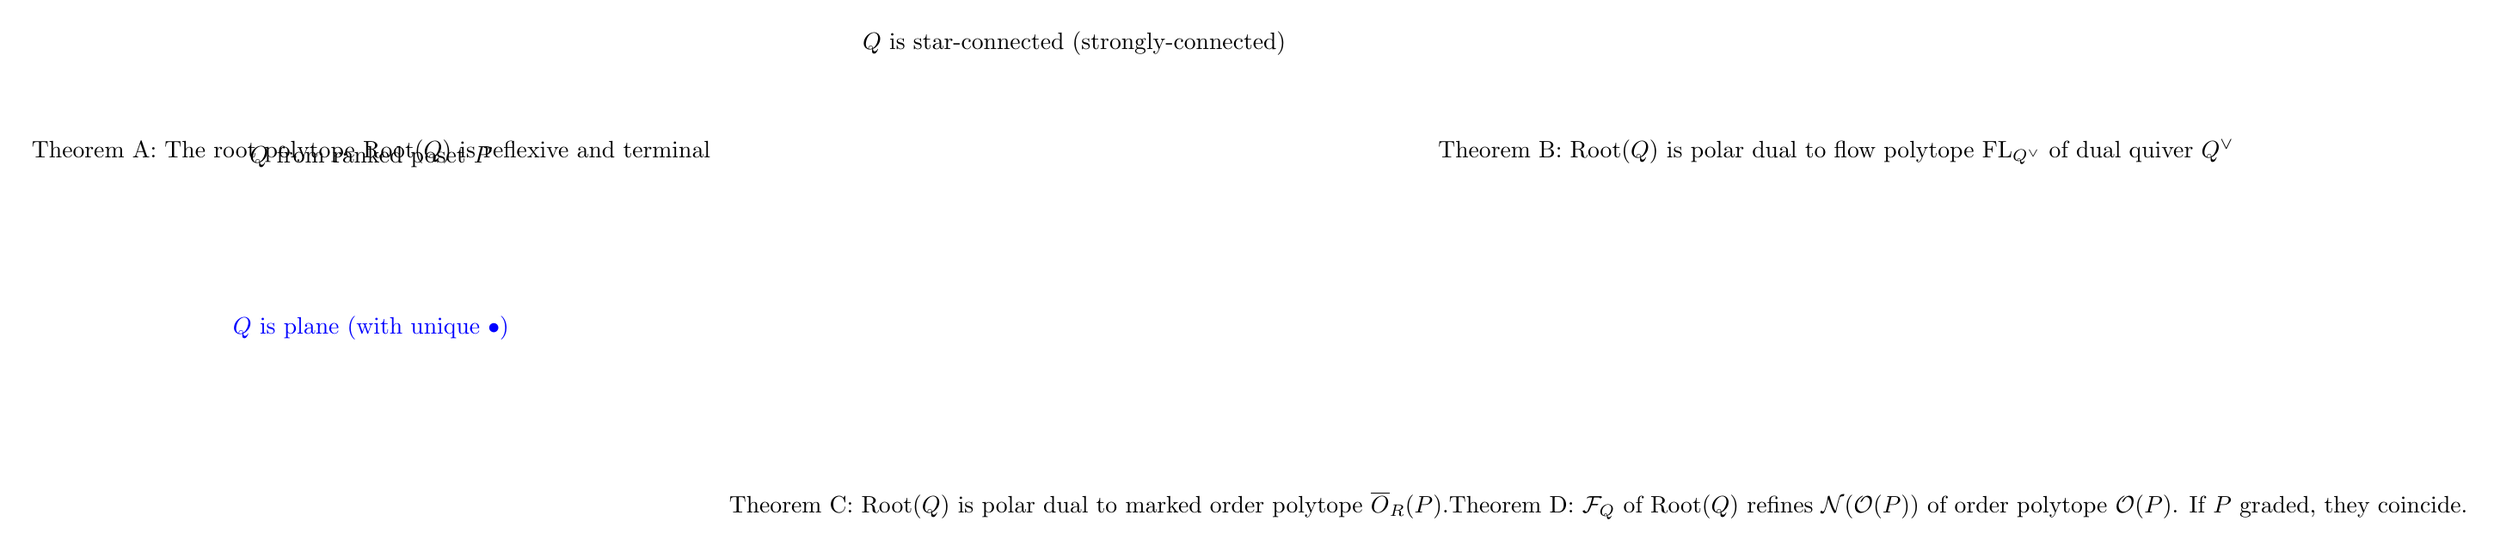
\begin{tikzpicture}[node distance=2cm, auto]
        \node (Q) {$ Q $ is star-connected (strongly-connected)};
        \node[below left = 1cm and 2cm of Q] (A) {Theorem A: The root polytope $\mathrm{Root}(Q)$ is reflexive and terminal};
        \node[below right = 1cm and 2cm of Q] (B) {Theorem B: $\mathrm{Root}(Q)$ is polar dual to flow polytope $\mathrm{FL}_{Q^{\vee}}$ of dual quiver $Q^{\vee}$};
        \node[below = 2cm of A, blue] (C) {$ Q $ is plane (with unique $\bullet$)};
        \node[below right = 2cm and 3cm of C] (D) {Theorem C: Root$(Q)$ is polar dual to marked order polytope $\overline{O}_R(P)$. \\ Theorem D: $\mathcal{F}_Q$ of $\mathrm{Root}(Q)$ refines $\mathcal{N}(\mathcal{O}(P))$ of order polytope $\mathcal{O}(P)$. If $P$ graded, they coincide.};
        \node[below = -0.5cm of A] (E) {$Q$ from ranked poset $P$};
    \end{tikzpicture}
\end{center}

\textbf{Overview of our main results}: they appear as \cref{cor:reflexive}, \cref{thm:dual}, \cref{prop:NPreflexive}, \cref{thm:refine}.

\end{document}